% Evidence-bounded RA-L submission candidate, 2026-09-24.
% Initial submission: two-column ieeeconf, US Letter, anonymous byline.
\documentclass[letterpaper,10pt,conference]{ieeeconf}
\IEEEoverridecommandlockouts
\overrideIEEEmargins

\usepackage{amsmath,amssymb}
\usepackage{graphicx}
\usepackage{booktabs}
\usepackage{cite}
\usepackage{flushend}
\usepackage{needspace}
\usepackage{url}
\usepackage{xcolor}
\usepackage{tikz}
\usetikzlibrary{arrows.meta,positioning,calc}

\definecolor{ink}{HTML}{183044}
\definecolor{teal}{HTML}{147D75}
\definecolor{amber}{HTML}{AD6423}
\definecolor{blue}{HTML}{27649E}
\definecolor{pale}{HTML}{F3F7F8}
\definecolor{warn}{HTML}{A94339}

\newcommand{\method}{BIND-VLA}
\newcommand{\policy}{\pi_{\theta}}

\begin{document}
\title{BIND-VLA: Boundary-Gated Agentic Supervision and Quality-Aware Inference}
\author{} % Keep the first submission anonymous.
\maketitle

\begin{abstract}
Frozen vision-language-action (VLA) policies can generate action chunks, but long-horizon manipulation also depends on remembering task context and deciding when a local action warrants correction. Adding an agentic supervisor creates a second problem: a premature override can interrupt useful motion, while repeated semantic inference can make the system slower. We present BIND-VLA, a harness that separates high-rate execution monitoring from lower-rate semantic decisions and admits ordinary subgoal changes only at action-chunk boundaries. Task-scoped memory supplies source-traceable context; an inference-profile gate considers replay validity, resource cost, and closed-loop quality before deployment. In an exploratory eight-task RoboMME study, success changes from 23/80 to 42/80 across development variants. A fixed identity-memory comparison on VideoUnmaskSwap changes 5/12 to 9/12, but transfer to VideoUnmask changes 15/16 to 13/16, and a frozen two-task Raw/Harness comparison changes 3/32 to 4/32. Separately, a PyTorch $\pi_{0.5}$ profile reduces model-call P95 latency from 282.43 to 54.67 ms on an RTX 4090. These results motivate controlled intervention and cost-aware deployment, while leaving general closed-loop gains and integrated acceleration unestablished.
\end{abstract}

\begin{keywords}
Vision-language-action models, embodied agents, robot manipulation, memory, efficient inference
\end{keywords}

\section{Introduction}
\label{sec:intro}
Vision-language-action (VLA) models connect language and perception to robot control, from OpenVLA to the $\pi_{0.5}$ family~\cite{openvla,pi05}. Their action chunks are local, however: a long task may require remembering a demonstrated target after occlusion, deciding whether a grasp or placement actually completed, and selecting the next skill. RoboMME makes such temporal and identity-dependent demands explicit~\cite{robomme}. Harness VLA suggests wrapping a frozen policy in higher-level capabilities~\cite{harnessvla}, but an external agent is not automatically helpful. Its decisions can be wrong, and its multimodal calls add latency even when the underlying policy is unchanged.

One failure in our development runs illustrates the control problem. A monitor treated gripper closure as evidence that a grasp had succeeded and switched the instruction to placement before the action was complete. The error was not in the VLA weights: a low-cost process signal had been granted authority over task semantics. Conversely, invoking a VLM after every action chunk can spend more time planning than acting. Faster model calls alone do not resolve this tradeoff; realtime VLA systems likewise distinguish network latency from continuous robot execution~\cite{realtimevla}.

We therefore ask: \emph{what evidence should authorize an agent to change a frozen policy's next subgoal, and at what runtime cost?} BIND-VLA separates a high-rate monitor, which reports execution signals, from a lower-rate vision-language model (VLM), which interprets task context. Task-scoped memory carries provenance rather than issuing actions. An authority gate checks semantic proposals and applies ordinary subgoal changes only at an action-chunk boundary; an independent safety interlock, when available, can still halt unsafe motion immediately. The frozen VLA remains the low-level controller. A separate profile gate screens policy inference configurations against latency, memory, replay validity, and task quality. Figure~\ref{fig:architecture} shows how these decisions surround, rather than replace, the action policy.

\begin{figure*}[t]
\centering
\resizebox{0.96\textwidth}{!}{\begin{tikzpicture}[x=1cm,y=1cm,>=Latex,font=\sffamily]
  \fill[blue!4] (0,3.57) rectangle (16.8,5.95);
  \fill[teal!4] (0,1.27) rectangle (16.8,3.36);
  \draw[ink!30,line width=0.5pt] (0,3.57) -- (16.8,3.57);
  \node[anchor=west,text=ink,font=\bfseries\scriptsize] at (0.16,5.73)
    {A. FROZEN ACTION LOOP};
  \node[anchor=west,text=ink,font=\bfseries\scriptsize] at (0.16,3.14)
    {B. EVIDENCE-GATED SUPERVISOR};

  \draw[blue!65,line width=0.8pt,fill=white] (0.25,3.83) rectangle (3.55,5.28);
  \node[inner sep=0pt] at (1.06,4.55)
    {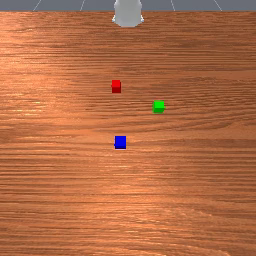
\includegraphics[width=1.24cm]{figures/ep39_demo.png}};
  \node[anchor=west,text=ink,font=\bfseries\scriptsize] at (1.78,4.81)
    {Observation $o_k$};
  \node[anchor=west,text=ink,font=\scriptsize] at (1.78,4.40)
    {RGB + state};
  \node[anchor=west,text=blue,font=\tiny] at (1.78,4.03)
    {recorded example};

  \draw[blue!65,line width=0.8pt,fill=white] (5.05,3.83) rectangle (8.38,5.28);
  \node[text=blue,font=\bfseries\small] at (6.72,4.74)
    {Frozen VLA $\pi_\theta$};
  \node[text=ink,font=\scriptsize] at (6.72,4.27)
    {fresh observation + subgoal};
  \node[text=amber,font=\tiny] at (6.72,3.99)
    {quality-admitted inference profile};

  \draw[blue!65,line width=0.8pt,fill=white] (9.17,3.83) rectangle (11.47,5.28);
  \node[text=blue,font=\bfseries\scriptsize] at (10.32,4.76)
    {Action chunk $A_k$};
  \node[text=ink,font=\scriptsize] at (10.32,4.30)
    {$a_{k,1},\ldots,a_{k,H}$};

  \draw[blue!65,line width=0.8pt,fill=white] (12.24,3.83) rectangle (16.55,5.28);
  \node[text=blue,font=\bfseries\scriptsize] at (14.40,4.78)
    {Robot / simulator};
  \node[text=ink,font=\scriptsize] at (14.40,4.35)
    {execute chunk; observe outcome};
  \node[text=ink,font=\tiny] at (14.40,4.01)
    {no semantic mid-chunk override};

  \draw[blue,->,line width=0.85pt] (3.58,4.56) -- (5.02,4.56);
  \draw[blue,->,line width=0.85pt] (8.41,4.56) -- (9.14,4.56);
  \draw[blue,->,line width=0.85pt] (11.50,4.56) -- (12.21,4.56);
  \draw[blue!75,->,line width=0.7pt] (14.40,5.30) -- (14.40,5.51)
    -- (1.90,5.51) -- (1.90,5.30);
  \node[fill=blue!4,inner sep=2pt,text=blue,font=\tiny] at (10.96,5.51)
    {next observation};

  \draw[teal!70,line width=0.8pt,fill=white] (0.25,2.20) rectangle (5.43,2.91);
  \node[anchor=west,text=teal,font=\bfseries\scriptsize] at (0.43,2.64)
    {Task memory};
  \node[anchor=west,text=ink,font=\scriptsize] at (2.10,2.64)
    {source frame $\cdot$ identity $\cdot$ provenance};
  \node[anchor=west,text=ink,font=\tiny] at (0.43,2.32)
    {historical evidence; re-ground target in the current frame};

  \draw[teal!70,line width=0.8pt,fill=white] (0.25,1.43) rectangle (5.43,2.12);
  \node[anchor=west,text=teal,font=\bfseries\scriptsize] at (0.43,1.86)
    {Execution monitor};
  \node[anchor=west,text=ink,font=\scriptsize] at (2.70,1.86)
    {risk + boundary receipt};
  \node[anchor=west,text=ink,font=\tiny] at (0.43,1.54)
    {process signals are not task-success certificates};

  \draw[teal!70,line width=0.8pt,fill=white] (6.04,1.43) rectangle (10.28,2.91);
  \node[text=teal,font=\bfseries\scriptsize] at (8.16,2.62)
    {Event-triggered VLM critic / planner};
  \node[text=ink,font=\scriptsize] at (8.16,2.17)
    {check scene and stage};
  \node[text=ink,font=\scriptsize] at (8.16,1.82)
    {propose a legal next subgoal};

  \draw[amber!85,line width=0.85pt,fill=white] (10.88,1.43) rectangle (16.55,2.91);
  \node[text=amber,font=\bfseries\scriptsize] at (13.72,2.62)
    {Boundary authority gate};
  \node[text=ink,font=\scriptsize] at (13.72,2.17)
    {freshness $\cdot$ allowlist $\cdot$ recovery budget};
  \node[text=ink,font=\scriptsize] at (13.72,1.82)
    {admit next subgoal or retain baseline};

  \draw[teal,->,line width=0.75pt] (5.46,2.54) -- (6.01,2.54);
  \draw[teal,->,line width=0.75pt] (5.46,1.78) -- (6.01,1.78);
  \draw[teal,->,line width=0.75pt] (10.31,2.20) -- (10.85,2.20);
  \draw[teal!70,->,line width=0.7pt] (2.92,3.80) -- (2.92,2.94);
  \draw[amber,->,line width=0.8pt] (13.63,2.94) -- (13.63,3.47)
    -- (6.72,3.47) -- (6.72,3.80);
  \node[fill=teal!4,inner sep=2pt,text=amber,font=\tiny] at (10.13,3.47)
    {only the next chunk};

  \draw[ink!30,line width=0.6pt] (0,0.0) rectangle (16.8,1.08);
  \node[anchor=west,text=ink,font=\bfseries\scriptsize] at (0.25,0.82)
    {C. TWO-RATE TIMELINE};
  \node[anchor=east,text=ink,font=\tiny] at (16.51,0.83)
    {profile admission: replay $\rightarrow$ call cost $\rightarrow$ paired quality};
  \foreach \xa/\xb/\lab in {3.20/6.25/$A_k$,6.63/9.68/$A_{k+1}$,10.06/13.11/$A_{k+2}$} {
    \fill[blue!12,draw=blue!70] (\xa,0.38) rectangle (\xb,0.68);
    \node[text=blue,font=\scriptsize] at ({(\xa+\xb)/2},0.53) {\lab};
  }
  \node[anchor=west,text=teal,font=\tiny] at (0.25,0.24)
    {monitor ticks};
  \draw[teal!60,line width=0.6pt] (3.20,0.17) -- (13.11,0.17);
  \foreach \x in {3.50,4.15,4.80,5.45,6.10,6.83,7.48,8.13,8.78,9.43,10.26,10.91,11.56,12.21,12.86}
    \draw[teal!65,line width=0.55pt] (\x,0.10) -- (\x,0.24);
  \fill[amber] (6.44,0.53) circle (0.09);
  \node[anchor=west,text=amber,font=\tiny] at (13.42,0.52)
    {semantic change only};
  \node[anchor=west,text=amber,font=\tiny] at (13.42,0.23)
    {at a boundary};
\end{tikzpicture}
}
\caption{BIND-VLA places checked semantic supervision around a frozen VLA action loop. A monitor reports process evidence; task memory and an event-triggered VLM supply context, but ordinary subgoal changes take effect only at a chunk boundary. A screened inference profile configures the policy call. The thumbnail is a recorded RoboMME demonstration frame; the evaluated GroundSG-skill adapter is narrower than the general interface.}
\label{fig:architecture}
\end{figure*}

Our contribution is a controlled way to compose agentic supervision with a
frozen action policy. We define a two-rate authority contract in which
execution signals can request review but cannot certify task completion or
rewrite an active chunk. We implement source-traceable memory and boundary
receipts, then measure both rescued and harmed paired episodes rather than
counting only successful recoveries. Finally, we couple the harness to a
quality-aware inference-profile gate and report model-call speed separately
from closed-loop cost. The evaluated evidence concerns one VLA family; it
does not establish online policy learning, hard realtime control, or
cross-policy generalization.

\section{Related Work}
\textbf{Planning, failure recovery, and memory.}
VLM-based correction and replanning are established in robotic manipulation:
ReplanVLM handles errors during task planning and execution~\cite{replanvlm},
while anomaly-triggered pause, perturbation, and reset have been tested on
physical robots~\cite{santhanam2026}. A hierarchical VLM/LLM planner with
learned action masks also addresses subtask switching without an extra
termination-model call~\cite{gu2026}. Harness VLA exposes frozen VLA behavior
as retryable capabilities~\cite{harnessvla}, and AHA uses a VLM to reason
about manipulation failures~\cite{aha}. We do not claim to invent semantic
replanning, detection, or recovery. BIND-VLA instead specifies when external
evidence may authorize the \emph{next} action chunk of an unchanged policy,
and audits rescues alongside harmful interventions. MemoryVLA embeds memory
in the policy~\cite{memoryvla}; our task-scoped records are external and
source-traceable. Long-horizon benchmarks such as CALVIN evaluate composed
language-conditioned behavior~\cite{calvin}; RoboMME provides the temporal
and identity-dependent tasks used here to test both memory benefit and
negative transfer~\cite{robomme}.

\textbf{Efficient execution and evaluation.}
TinyVLA improves speed through a compact policy architecture~\cite{tinyvla}.
PointVLA keeps an action expert frozen but learns a lightweight 3D feature
injection module~\cite{pointvla}; BIND-VLA instead leaves the policy weights
and representations unchanged. This preserves a plug-in control interface
but cannot itself repair missing visual features. Realtime VLA systems
address policy inference and action continuity
~\cite{realtimevla,realtimevlav2,realtimeflash}. RILaaS measures inference
serving under robot deployment loads~\cite{rilaas}, illustrating why
model-call latency and full execution cost must be reported separately.
Our profile study combines existing backend settings with a paired-quality
admission rule, rather than proposing compilation, quantization, or a new
VLA backbone. LIBERO-PRO probes robustness beyond memorized LIBERO
trajectories~\cite{liberopro}; our local ten-state subset is not its official
leaderboard protocol.

\section{Agentic Execution and Inference Control}
\label{sec:method}
\subsection{Execution authority at action boundaries}
At chunk boundary $k$, let $o_k$ be deployable visual/proprioceptive observations, $\ell$ the task instruction, $m_k$ a bounded memory record, and $b_k$ the remaining call/recovery budget. The frozen policy proposes a chunk
\begin{equation}
 A_k=\policy(o_k,\ell_k)=(a_{k,1},\ldots,a_{k,H}).
\end{equation}
The controller executes the admitted portion, collects a receipt $e_k$ from the robot/simulator adapter, and updates its state only from observations and receipts. Evaluator success flags, online oracle subgoals, and privileged simulator object poses are excluded from decisions. The monitor can flag stalling, action age, deadline failures, or inconsistent progress. Such a flag is a \emph{request for review}, not proof of grasp or subtask completion.

In the reusable runtime, an escalated VLM decision has one typed intent from $\{\texttt{continue},\texttt{vla\_act},\texttt{run\_skill},\texttt{safe\_stop}\}$. The gate checks schema, freshness, capability allowlist, and budget. Memory may supply object identity and provenance but cannot issue joint commands; the VLM may select a textual subgoal or registered skill, not torques or trajectories. The RoboMME evaluation uses a narrower adapter: its GroundSG planner returns task-specific language subgoals, which are checked against the legal skill grammar and fail closed on invalid output. Thus the paired RoboMME results test boundary receipts and memory on one PI0.5/VLM chain, not every typed tool of the general runtime. The policy-adapter interface is replaceable, but cross-policy performance is untested.

\subsection{Memory, stage state, and non-interruption}
The memory record is indexed by task and episode and carries source observation, target identity, and provenance. Admission checks its task scope and source; the VLM must re-ground a historical target in the live frame. An ordered stage state separates local motion from task completion: gripper closure is an execution signal, not proof of a correct grasp. The controller never rewrites a running action chunk on this signal alone. At the next boundary, it can present an execution receipt to the VLM and request a legal next skill, retry within budget, or stop. This corrects an earlier monitor/planner authority inversion without asserting that a receipt alone verifies successful placement.

For the VideoUnmask task family, an offline compiler uses only the public
initial demonstration. It detects color-coded cubes before occlusion and
their nearest white containers at the first covered frame, rejecting
associations beyond 20 pixels. SAM~2~\cite{sam2} tracks each associated
container to the end of the video; excessive mask loss rejects the record.
The retained color-to-container map, requested order, and source-video hash
are passed to the VLM as \emph{historical evidence}, not as verified current
positions or completion flags. The VLM must still ground the next target in
the live frame. Compilation time is accounted for separately from rollout
latency.

\subsection{Selective semantic calls and profile admission}
Let $r_k$ denote monitor risk and $v_k$ indicate whether a cached subgoal remains valid under the new observation. A VLM call is requested when an event is raised, the cached subgoal is invalid, or its reuse budget expires. Otherwise the current subgoal is reused and the policy sees a fresh $o_k$; \emph{only the semantic plan is cached, not the action chunk}. In the current implementation, validation and fallback occur at chunk boundaries rather than by speculative mid-chunk commands. This distinction matters because an apparently faster scheduler can reduce episode duration simply by failing earlier.

Writing $E_k$ for an event raised from $r_k$ or a task-state change and $c_k$
for the remaining reuse count, the
semantic-call proposal is
\begin{equation}
 q_k=\mathbb{1}\{E_k\lor\neg v_k\lor c_k=0\}.
\end{equation}
Regardless of $q_k$, a new low-level chunk is generated from the current
observation. If $q_k=1$, the returned semantic intent must pass the authority
gate before it can change the \emph{next} subgoal; it never rewrites a chunk
already executing.

For deployment accounting, we distinguish policy computation from the rest
of the control loop. Per-episode wall time comprises observation handling,
VLA calls, semantic VLM calls, synchronization, and environment or robot
execution. This is an accounting identity, not five independently measured
timings in every experiment. Selective VLM calls can reduce one term while
increasing policy calls or prolonging a trajectory; quality-admitted profiles
must therefore be checked against \emph{complete} paired episodes, not only
single-call P95.

An inference profile identifies checkpoint, backend, precision, flow-step count, view mask, action horizon, and target hardware. Admission has three gates: matched-output replay, warm single-call latency and memory under a declared budget, and paired closed-loop task quality. A profile that meets a latency target but worsens task quality is rejected or retained only for a separately labeled low-memory tier. The reported 80-ms threshold below is a \emph{model-call target}, not a guarantee on sensing, planning, and robot actuation together.
In particular, a candidate is not deployed merely because its measured
$T_{95}$ is lower: it must also meet the predeclared paired-quality rule
$Q(P)\geq Q(P_0)-\epsilon$ and the memory budget. In our conservative
screens, an observed harm can reject a candidate even when the mean
success difference is small; this sample gate is not a population-level
non-inferiority test.

\section{Experimental Protocol}
\label{sec:protocol}
We separate three non-interchangeable experimental settings. The historical RoboMME study uses the official GroundSG PI0.5 checkpoint 79999 and a Qwen3-VL-4B GroundSG planner, 16-action chunks, and a 1300-step limit. Eight of RoboMME's 16 tasks are covered with 10 fixed episodes per task and condition. B1 invokes the planner every chunk without harness memory/tools; C2 adds memory, grounded tools, and procedure/temporal control while retaining every-chunk planning; C3 adds selective planning and validated subgoal reuse. The same task/episode identities are paired. All success values are official environment outcomes. This is a \emph{historical development-and-expansion study}: C3 aggregates several task-specific development revisions, and the last four tasks were added after the first four had been studied. The nominal paired statistics below therefore describe the recorded sample; they are not a pre-registered confirmation of one frozen final implementation.

To isolate identity memory on the same action-policy and VLM chain, a later
VideoUnmaskSwap gate preselected episodes 30--37, followed by a separately
preselected confirmation range 38--53. The official test split has only 50
episodes: four out-of-range IDs 50--53 returned duplicate preflight states
and were excluded \emph{before any model rollout}, without replacement.
The confirmation therefore has 12 valid, previously unused paired states, 38--49.
A retains the full public initial demonstration but no structured memory;
B adds only color-to-container identity memory compiled from that same
demonstration. Both arms use the same frozen models, 16-step chunks, camera,
planner-at-every-chunk schedule, 1300-step budget, and model-service start;
order alternates A--B and B--A by episode parity. Stage-receipt and
identity-conflict corrections are disabled. Rejected memories and all official
failures, including budget-exhausted ongoing runs, are retained.

For task outcomes, we report both total successes and paired transitions: a \emph{rescue} means the baseline failed and the compared method succeeded on the same task/episode, whereas a \emph{regression} reverses that outcome. A recovery event within one rollout is not automatically a rescue. Exact McNemar tests use only discordant paired outcomes. Planner calls, policy calls, and elapsed wall time are recorded separately, since reducing one count does not imply an end-to-end speedup. We distinguish all-episode totals from the cost of \emph{both-successful} pairs; the latter avoids calling an early failure ``fast.''

The separate LIBERO experiment uses a PyTorch PI0.5 LIBERO checkpoint and Qwen3.5-4B semantic planner. Four locally available ten-task suites (standard LIBERO-10 and three LIBERO-PRO variants) are evaluated on 10 initial states per task, 400 paired states per condition. This is not the official 50-initial-state leaderboard. Finally, the model-call experiment uses the same PyTorch PI0.5 family on an RTX 4090 and 45 paired recorded observations with fixed noise and action horizon 10. Its numbers must not be transferred to the RoboMME JAX implementation.

\section{Results and Evidence Boundaries}
\label{sec:results}
\subsection{Exploratory long-horizon study}
Table~\ref{tab:robomme} contains the complete historical eight-task aggregate. Relative to B1, C2 has 18 failure-to-success and 5 success-to-failure transitions; C3 has 22 and 3. The corresponding nominal exact McNemar $p$ values are 0.0106 and 0.000157. Because C3 includes development variants, these values should not be interpreted as confirmatory significance for the final harness. Relative to C2, C3 saves 813 planner calls (40.6\%) and 1455.2 seconds of cumulative wall time (28.1\%) but makes more policy calls (2169 versus 2001); its six-success advantage has nominal $p=0.146$. Cost and task quality must be read together.

\begin{table}[t]
\caption{Historical RoboMME study: eight tasks, 80 paired episodes per arm. These are exploratory development/expansion results, not one frozen confirmation run.}
\label{tab:robomme}
\centering\footnotesize
\begin{tabular}{lrrrr}
\toprule
Condition & Success & Planner & Policy & Wall (s)\\
\midrule
B1 Raw & 23/80 & 2141 & 2141 & 5208.0\\
C2 Harness & 36/80 & 2001 & 2001 & 5178.7\\
C3 + selective & 42/80 & 1188 & 2169 & 3723.6\\
\bottomrule
\end{tabular}
\end{table}

\begin{table}[t]
\caption{Task-level RoboMME successes (of 10 each). Heterogeneity matters: the strongest gains are not uniform across tasks.}
\label{tab:tasks}
\centering\footnotesize
\begin{tabular}{lrrr}
\toprule
Task & B1 & C2 & C3\\
\midrule
StopCube & 0 & 3 & 2\\
VideoRepick & 2 & 3 & 7\\
RouteStick & 1 & 3 & 5\\
VideoUnmaskSwap & 2 & 7 & 8\\
BinFill & 7 & 8 & 8\\
ButtonUnmask & 0 & 3 & 2\\
PickHighlight & 3 & 2 & 2\\
MoveCube & 8 & 7 & 8\\
\bottomrule
\end{tabular}
\end{table}

The historical B1-to-C2 transition has five harms alongside 18 rescues. C2-to-C3, which isolates scheduling more closely, has nine rescues and three harms; its nominal test does not establish that the scheduler improves success. C3 also makes 168 more low-level policy calls than C2. Thus fewer planner calls do not imply faster policy inference or a uniformly better controller.

The four later-added tasks yield 18/40, 20/40, and 20/40 for B1/C2/C3.
Earlier Swap development screens varied across service starts; neither
they nor this aggregate establish a frozen multi-task effect.

\subsection{Fixed identity-memory gate and within-task confirmation}
Table~\ref{tab:memory} isolates public-demonstration identity memory rather
than the full multi-module harness. All eight gate and twelve valid
confirmation memories pass the admission check; every A/B pair has matching
initial-observation hashes and runs within one service start. Confirmation
yields five rescues and one harm, a descriptive 33.3-point success difference
but exact two-sided McNemar $p=0.21875$. Three rescues occur in six
single-target tasks; the six two-target tasks have two rescues and one harm.
This is directional within-task evidence, not statistical significance or
cross-task generalization.

\begin{table}[t]
\caption{RoboMME identity-memory A/B. A sees the public demonstration; B additionally receives tracked identity memory. Official success; budget exhaustion counts as non-success. Unmask is a separate transfer test.}
\label{tab:memory}
\centering\footnotesize
\setlength{\tabcolsep}{4pt}
\begin{tabular}{lrrrr}
\toprule
Set & A success & B success & Rescues & Harms\\
\midrule
Swap gate ep30--37 & 2/8 & 4/8 & 2 & 0\\
Swap confirm ep38--49 & 5/12 & 9/12 & 5 & 1\\
Unmask ep22--37 & 15/16 & 13/16 & 1 & 3\\
\bottomrule
\end{tabular}
\end{table}

\begin{figure}[t]
\centering
\resizebox{0.96\columnwidth}{!}{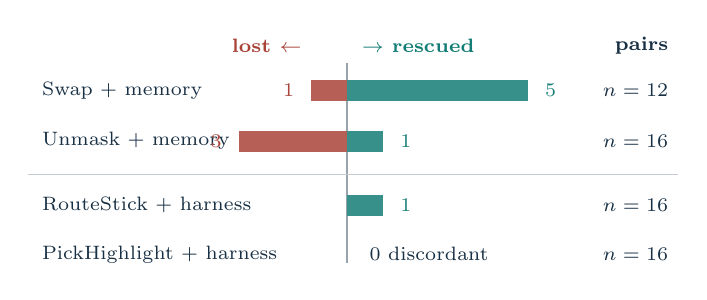
\begin{tikzpicture}[x=1cm,y=1cm,font=\scriptsize]
  \node[anchor=west,text=warn,font=\bfseries\scriptsize] at (2.51,3.13)
    {lost $\leftarrow$};
  \node[anchor=west,text=teal,font=\bfseries\scriptsize] at (4.16,3.13)
    {$\rightarrow$ rescued};
  \node[anchor=east,text=ink,font=\bfseries\scriptsize] at (8.30,3.13)
    {pairs};
  \draw[ink!45,line width=0.65pt] (4.10,0.37) -- (4.10,2.91);
  \draw[ink!25,line width=0.5pt] (0.05,1.49) -- (8.30,1.49);

  \node[anchor=west,text=ink] at (0.10,2.56) {Swap + memory};
  \fill[warn!85] (3.64,2.42) rectangle (4.10,2.69);
  \fill[teal!85] (4.10,2.42) rectangle (6.40,2.69);
  \node[anchor=east,text=warn] at (3.55,2.56) {1};
  \node[anchor=west,text=teal] at (6.49,2.56) {5};
  \node[anchor=east,text=ink] at (8.30,2.56) {$n=12$};

  \node[anchor=west,text=ink] at (0.10,1.92) {Unmask + memory};
  \fill[warn!85] (2.72,1.78) rectangle (4.10,2.05);
  \fill[teal!85] (4.10,1.78) rectangle (4.56,2.05);
  \node[anchor=east,text=warn] at (2.63,1.92) {3};
  \node[anchor=west,text=teal] at (4.65,1.92) {1};
  \node[anchor=east,text=ink] at (8.30,1.92) {$n=16$};

  \node[anchor=west,text=ink] at (0.10,1.10) {RouteStick + harness};
  \fill[teal!85] (4.10,0.96) rectangle (4.56,1.23);
  \node[anchor=west,text=teal] at (4.65,1.10) {1};
  \node[anchor=east,text=ink] at (8.30,1.10) {$n=16$};

  \node[anchor=west,text=ink] at (0.10,0.48) {PickHighlight + harness};
  \node[anchor=west,text=ink] at (4.26,0.48) {0 discordant};
  \node[anchor=east,text=ink] at (8.30,0.48) {$n=16$};
\end{tikzpicture}
}
\caption{Direction of outcome changes in fixed RoboMME pairs. Left bars count baseline successes lost; right bars count baseline failures rescued. Memory rows isolate demonstration-derived identity; harness rows compare frozen Raw and Harness configurations. The tasks were selected for targeted tests, not as an unbiased RoboMME average.}
\label{fig:paired}
\end{figure}

Figure~\ref{fig:qualitative} shows Swap confirmation ep39. After the first placement, B grounds the red-hidden
second container near $(98,94)$ and succeeds; A repeatedly targets around
$(81,112)$ and fails. This is consistent with identity memory changing the
semantic target. The paired Swap counterexample ep43 follows the correct
green-to-blue order in both arms, yet B fails and A succeeds. Identity
correctness does not guarantee the physical action trajectory. Moreover,
rescued Swap ep47 requires 1075 steps and 68 VLM/policy calls with B, so a higher
completion count cannot be read as lower deployment cost. On only four
both-successful confirmation pairs, A/B use 46/43 planner calls and
60.47/57.91 seconds; these differing trajectories provide no evidence for
the separate Optimize Runtime's effect.

\begin{figure*}[t]
\centering
\begin{minipage}{0.28\textwidth}\centering
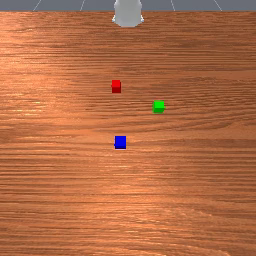
\includegraphics[width=\linewidth]{figures/ep39_demo.png}\\[-1pt]
\footnotesize Public initial demonstration
\end{minipage}\hfill
\begin{minipage}{0.28\textwidth}\centering
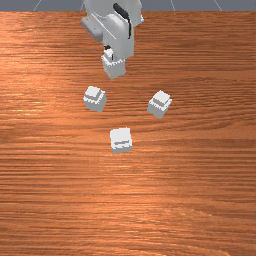
\includegraphics[width=\linewidth]{figures/ep39_no_memory_final.png}\\[-1pt]
\footnotesize A: no identity memory; failure
\end{minipage}\hfill
\begin{minipage}{0.28\textwidth}\centering
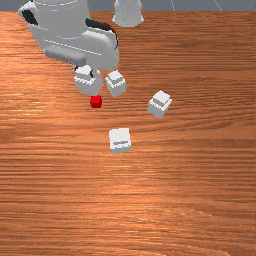
\includegraphics[width=\linewidth]{figures/ep39_memory_final.png}\\[-1pt]
\footnotesize B: identity memory; success
\end{minipage}
\caption{Qualitative paired VideoUnmaskSwap episode 39. The left frame is
from the public demonstration; the other frames are the terminal top-view
rollout images, not synchronized counterfactual states. A's final VLM target
is $(80,112)$ and it fails; B's is $(98,93)$ and it succeeds. This illustrates
how demonstration-derived identity can change a later target, but is one
case, not a population-level effect estimate.}
\label{fig:qualitative}
\end{figure*}

The fixed second-task transfer test uses 16 previously unused VideoUnmask
episodes and the same public-video SAM2 compiler. Unlike an earlier pilot in
which a motion gate suppressed all memory hints, B now actually receives the
admitted identity record in every episode. A/B succeed in 15/16 and 13/16
respectively (one rescue, three harms; exact two-sided $p=0.625$). All twelve
single-target pairs succeed in both arms, while success on four two-target
pairs changes from 3/4 to 1/4. In two harms, B repeatedly attempts the first
pickup; another exhausts its 1300-step budget in a placement loop. Thus a
correctly sourced identity record does not ensure robust stage execution.
The twelve both-successful pairs use 134 versus 100 planner/policy calls and
152.74 versus 121.41 seconds, but differing trajectories and the omitted
SAM2 build cost (21.67 seconds for these pairs, excluding shared model load)
preclude an unconditional efficiency claim. Always-on transfer is rejected.
An additional matched Unmask development pilot (ep38--45) yields 8/8,
8/8, and 7/8 for Raw, observation-only Harness, and Harness+memory:
no rescue and one harm. We then added an opt-in boundary receipt recording
that a put-down chunk ran and naming the next demonstration target; it
neither certifies placement nor interrupts that chunk. The pilot's failed
ep43 succeeds on rerun (365 steps), a targeted repair rather than an
independent rescue. On unseen two-target ep47, frozen Raw, Harness, and
Harness+memory+receipt all succeed (313, 313, and 327 steps). This tests
the receipt path but shows no success-rate or efficiency gain.

A same-chain B/C ablation asks whether selective VLM scheduling can mitigate
this overhead without losing task quality. Using the same memory and models,
B plans every chunk and C uses validated subgoal reuse. On eleven strict
same-service pairs, B/C succeed in 8/11 and 7/11, with one rescue and two
harms. In the six both-successful pairs, planner calls fall from 45 to 29
and total wall time from 66.84 to 52.13 seconds, while policy calls change
from 45 to 44. Yet the predeclared quality gate rejects C because of the
two harms. In the twelfth episode, C proposes an unsupported action skill
and is safely rejected at 112 steps; B is completed in a second service
start and succeeds. This cross-service case is excluded from strict paired
quality and timing totals, and the C error is not relabeled as an official
task failure. These observations demonstrate an overhead--quality tradeoff,
not an admitted Optimize profile.

\subsection{Frozen Raw/Harness task stress test}
To assess whether the current implementation reproduces the exploratory
multi-task trend, we fix two task families selected for opposing historical
behavior: RouteStick previously improved, while PickHighlight had a
regression. On 16 new paired episode identities per task, both arms use the
same GroundSG PI0.5, Qwen3-VL, observations, and every-chunk schedule;
Harness alone adds its existing task-specific planning contract, without
identity memory or the rejected selective schedule. RouteStick yields
Raw/Harness success of 0/16 versus 1/16; PickHighlight yields 3/16 versus
3/16. Combined, the frozen comparison is 3/32 versus 4/32, one rescue,
zero harms, exact two-sided McNemar $p=1$. Three pairs succeed under both
arms; their combined wall time is 53.43 versus 55.01 seconds and planner/
policy calls 58 versus 60. Two Harness runs exhaust the control budget,
compared with one Raw run. The task families were purposefully chosen from
historical positive and regression cases, not randomly sampled from RoboMME;
their poor absolute success also limits how much high-level supervision can
be assessed. The fixed test therefore bounds the exploratory result: it
does not show a strong Harness gain or whole-system acceleration.

\subsection{LIBERO robustness and agent overhead}
On 400 locally paired states, frozen PI0.5 succeeds 180 times, fixed recovery 181, and the agentic variant 183. The frozen-to-agentic difference is 0.75 percentage points (four rescues, one regression; exact McNemar $p=0.375$). VLA calls fall from 16047 to 14699 (8.4\%), but cumulative wall time rises from 7610.7 to 8864.6 seconds (16.5\%) as 263 semantic-planning calls are added. The clean LIBERO-10 subset is already 96/100 for the frozen policy, whereas the more perturbed Swap and Task subsets remain 11/100 and 7/100 for both frozen and agentic conditions (Table~\ref{tab:libero}). This experiment supports a concrete systems motivation---the semantic layer can dominate total cost---but not a broad success or end-to-end speed claim.

\begin{table}[t]
\caption{LIBERO local ten-state subset by suite; each row is 10 tasks $\times$ 10 states. Not official 50-state leaderboard scores.}
\label{tab:libero}
\centering\footnotesize
\begin{tabular}{lrrr}
\toprule
Suite & Frozen & Fixed & Agentic\\
\midrule
LIBERO-10 & 96/100 & 97/100 & 97/100\\
Object perturbation & 66/100 & 67/100 & 68/100\\
Swap perturbation & 11/100 & 11/100 & 11/100\\
Task perturbation & 7/100 & 6/100 & 7/100\\
\bottomrule
\end{tabular}
\end{table}

\subsection{Independent inference-profile measurements}
Figure~\ref{fig:runtime} reports single-call P95 on 45 paired recorded observations. The 7-step eager and 2-step compiled profiles differ in both flow-step count and backend, so their ratio is not attributable to one optimization. Within the 2-step configurations, compilation and static masked-view elision (SMVE) further lower measured latency. The current late-language INT8 route saves memory but is too slow and is rejected. Fidelity checks on 45 records for V2--V4 concern the defined replay comparison; they do not prove that 7-step and 2-step policies have equal closed-loop quality.

\begin{figure}[t]
\centering
\resizebox{0.96\columnwidth}{!}{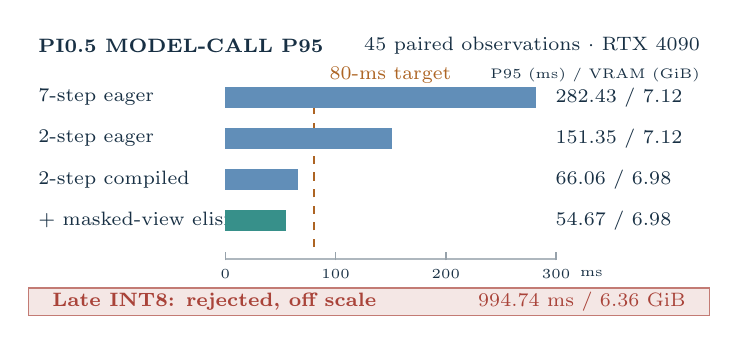
\begin{tikzpicture}[x=1cm,y=1cm,font=\sffamily]
  \node[anchor=west,text=ink,font=\bfseries\scriptsize] at (0.10,3.60)
    {PI0.5 MODEL-CALL P95};
  \node[anchor=east,text=ink,font=\scriptsize] at (8.75,3.60)
    {45 paired observations $\cdot$ RTX 4090};
  \draw[ink!35,line width=0.6pt] (2.60,0.89) -- (6.80,0.89);
  \foreach \x/\lab in {2.60/0,4.00/100,5.40/200,6.80/300} {
    \draw[ink!45,line width=0.5pt] (\x,0.87) -- (\x,0.98);
    \node[text=ink,font=\tiny] at (\x,0.70) {\lab};
  }
  \node[anchor=west,text=ink,font=\tiny] at (6.98,0.70) {ms};
  \draw[amber,dashed,line width=0.75pt] (3.72,1.04) -- (3.72,3.12);
  \node[anchor=west,text=amber,font=\scriptsize] at (3.80,3.23)
    {80-ms target};

  \node[anchor=west,text=ink,font=\scriptsize] at (0.10,2.94)
    {7-step eager};
  \fill[blue!73] (2.60,2.81) rectangle (6.55,3.07);
  \node[anchor=west,text=ink,font=\scriptsize] at (6.67,2.94)
    {282.43 / 7.12};

  \node[anchor=west,text=ink,font=\scriptsize] at (0.10,2.42)
    {2-step eager};
  \fill[blue!73] (2.60,2.29) rectangle (4.72,2.55);
  \node[anchor=west,text=ink,font=\scriptsize] at (6.67,2.42)
    {151.35 / 7.12};

  \node[anchor=west,text=ink,font=\scriptsize] at (0.10,1.90)
    {2-step compiled};
  \fill[blue!73] (2.60,1.77) rectangle (3.52,2.03);
  \node[anchor=west,text=ink,font=\scriptsize] at (6.67,1.90)
    {66.06 / 6.98};

  \node[anchor=west,text=ink,font=\scriptsize] at (0.10,1.38)
    {+ masked-view elision};
  \fill[teal!85] (2.60,1.25) rectangle (3.37,1.51);
  \node[anchor=west,text=ink,font=\scriptsize] at (6.67,1.38)
    {54.67 / 6.98};

  \draw[warn!70,line width=0.6pt] (0.10,0.17) rectangle (8.75,0.52);
  \fill[warn!13] (0.11,0.18) rectangle (8.74,0.51);
  \node[anchor=west,text=warn,font=\bfseries\scriptsize] at (0.28,0.35)
    {Late INT8: rejected, off scale};
  \node[anchor=east,text=warn,font=\scriptsize] at (8.57,0.35)
    {994.74 ms / 6.36 GiB};
  \node[anchor=east,text=ink,font=\tiny] at (8.75,3.23)
    {P95 (ms) / VRAM (GiB)};
\end{tikzpicture}
}
\caption{Independent PyTorch PI0.5 model-call profiles on RTX 4090 (45 paired observations). The dashed line is an 80-ms \emph{call} target; INT8 is separately labeled because its 994.74-ms P95 exceeds the plotted range. Different step counts cannot be credited to compilation alone. These are not end-to-end JAX RoboMME timings.}
\label{fig:runtime}
\end{figure}

For Qwen3.5-4B, NF4 reduces allocated model memory from 8.46 to 3.08 GiB while increasing P95 from 1896.55 to 2909.79 ms. Thirty recorded semantic cases agree exactly; this is a memory tier, not a latency optimization. One co-resident NF4-planner/SMVE-policy smoke test occupies 11.22 GiB but withholds robot actions; it demonstrates model integration only.

There is a limited closed-loop profile gate on two saved recovery snapshots (tasks 06 and 09) from the PyTorch LIBERO line. Compile+SMVE BF16 succeeds on both; late-language INT8 alone also succeeds on both but is slower and thus only a lower-memory option. The composed INT8+SMVE profile fails one of the two and is rejected. These branches test a fixed physical-recovery continuation, \emph{not} the VLM-guided Agentic Harness, and two snapshots do not estimate population-level task success. They do, however, show why a profile should be admitted by quality as well as by isolated latency.

\section{Discussion and Limitations}
The central systems variable is \emph{intervention authority}. Gripper
closure and other inexpensive signals can flag risk without proving that a
subtask is complete. A source-correct identity mapping can still harm a
rollout if stage execution is wrong: Swap memory rescues five confirmation
pairs but loses one, and always-on Unmask transfer loses three. The monitor
can therefore run frequently while semantic changes wait for a fresh image,
a VLM decision, and the next chunk boundary. The repaired Unmask ep43 shows
that this path is executable; unseen ep47 shows that it need not be faster.

These observations do not establish a statistically robust gain for a
frozen integrated system. The eight-task aggregate mixes development
revisions, the identity-memory confirmation is non-significant
($p=0.21875$), and a retrospective motion check remains untested in
closed loop. Selective planning fails its paired quality gate even where
both-successful trajectories use fewer calls. Initial-state matching
does not prevent later trajectories from diverging. The PyTorch PI0.5
profile is a separate model-call result, not acceleration of the JAX
RoboMME robot chain. We test one action-policy family, without a physical
robot. In contrast, recent RA-L recovery and hierarchical-execution studies
include physical-robot or cross-platform tests~\cite{santhanam2026,gu2026};
our simulator-only evidence does not meet that validation standard. A
submission-strength integrated claim still needs a frozen
multi-task comparison and a quality-admitted, same-chain Optimize profile.

\section{Conclusion}
BIND-VLA treats agentic intervention as an authority-and-budget decision around
a frozen VLA. Boundary-timed supervision prevents inexpensive process signals
from directly rewriting an active action chunk. In paired tests,
source-traceable memory helps one identity-dependent task but harms blind
transfer, and the frozen Raw/Harness comparison shows only a small change.
Separately, quality-screened profiles reduce PI0.5 model-call latency, not
the measured JAX robot-chain time. The resulting design supports
conditional, auditable supervision; its joint task-quality and efficiency
benefit remains to be established in a frozen multi-task test.

\bibliographystyle{ieeetr}
\bibliography{references}
\end{document}
